\section{Résultats et évaluation du pipeline}
\begin{frame}
    \frametitle{Résultats: effet des itérations et du batch}
    \begin{columns}[T,totalwidth=\textwidth]
        \column{0.5\textwidth}
        \centering
        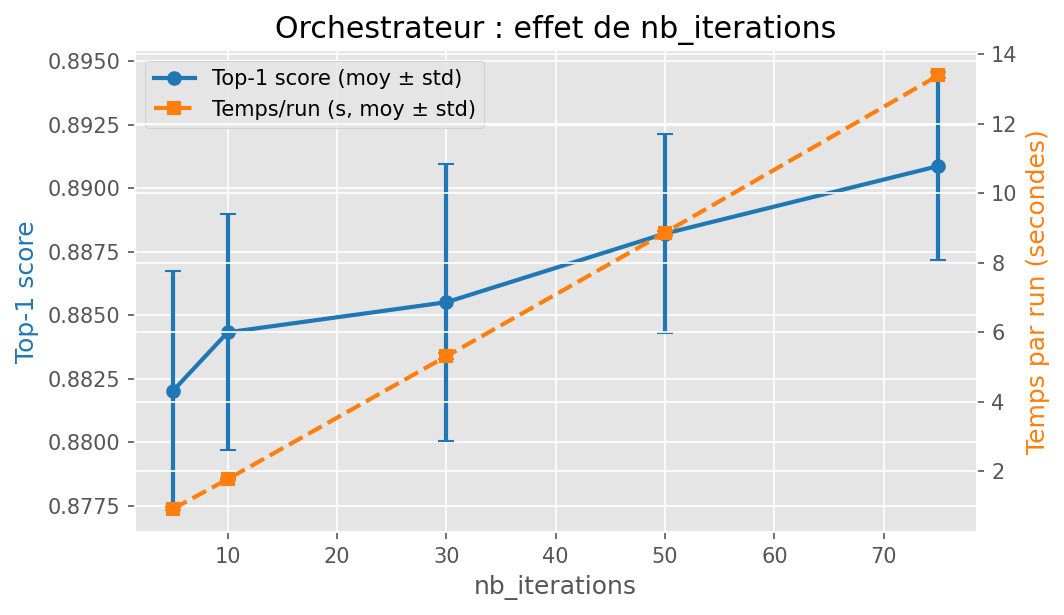
\includegraphics[width=\linewidth]{images/nb_iterations.png}

        \column{0.5\textwidth}
        \centering
        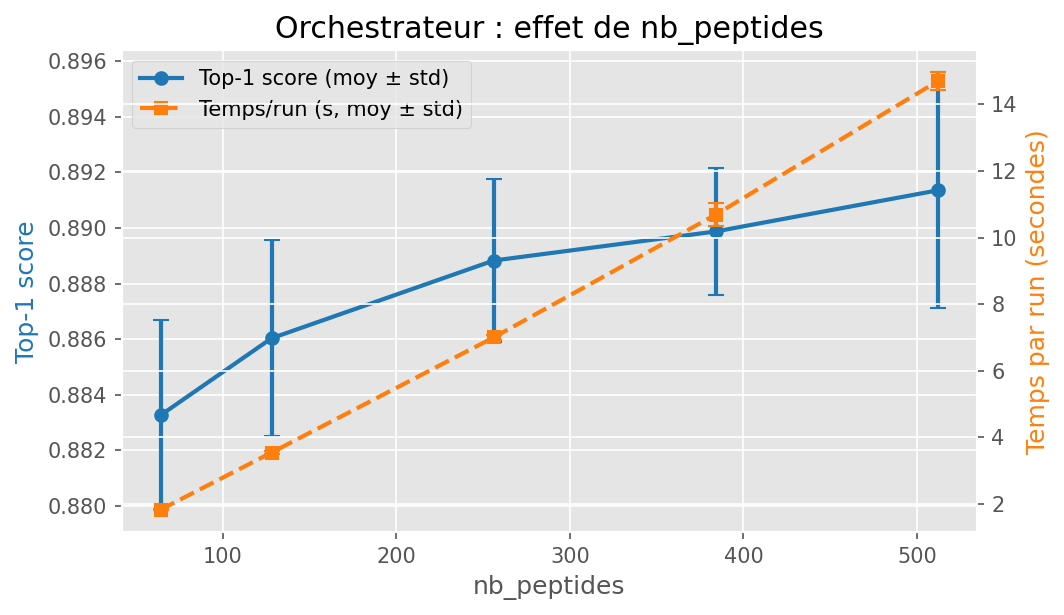
\includegraphics[width=\linewidth]{images/nb_peptides.png}
    \end{columns}

    \vspace{0.3em}
    \begin{block}{Message clé}
        \footnotesize
        Plus d'itérations et plus de peptides par round augmentent très légèrement le score, mais le temps d'exécution augmente fortement..
    \end{block}
\end{frame}

\begin{frame}
    \frametitle{Résultats: impact de la longueur cible}
    \begin{columns}[T,totalwidth=\textwidth]
        \column{0.60\textwidth}
        \centering
        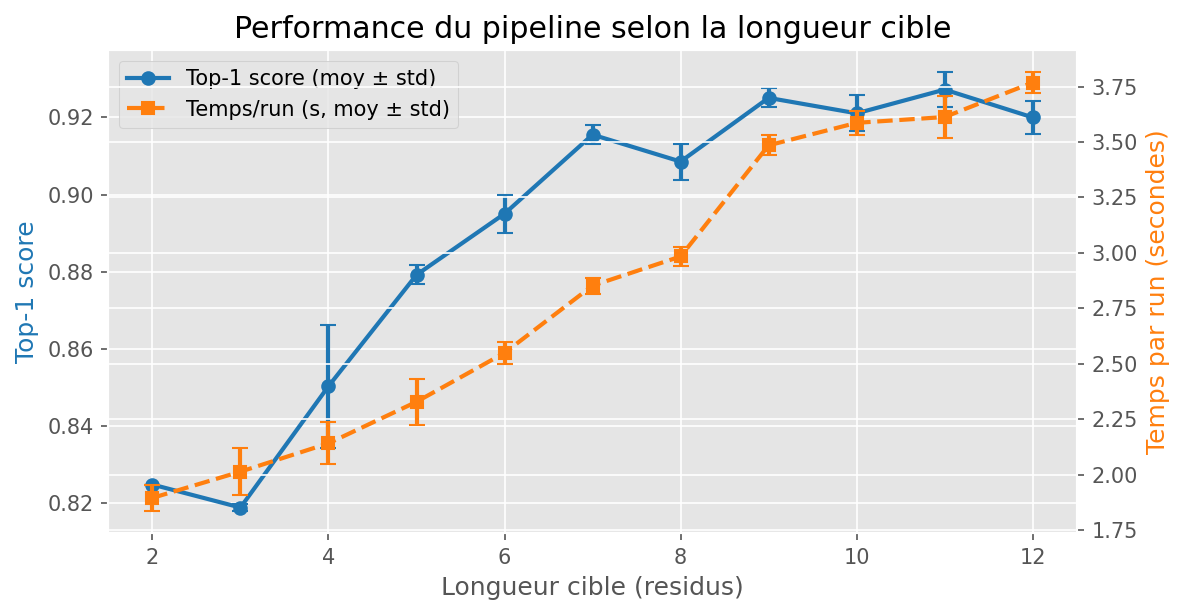
\includegraphics[width=\linewidth]{images/target_length.png}

        \column{0.36\textwidth}
        \begin{block}{Analyse}
            \footnotesize
            \begin{itemize}
                \item Les cibles très courtes (2--3) sont les plus difficiles.
                \item Le score augmente puis se stabilise autour de $\sim 0.92$ pour des longueurs plus grandes.
                \item Le runtime monte de façon modérée.
            \end{itemize}
        \end{block}
    \end{columns}
\end{frame}

\begin{frame}
    \frametitle{Pipeline vs baseline (score et diversité)}
    \begin{columns}[T,totalwidth=\textwidth]
        \column{0.5\textwidth}
        \centering
        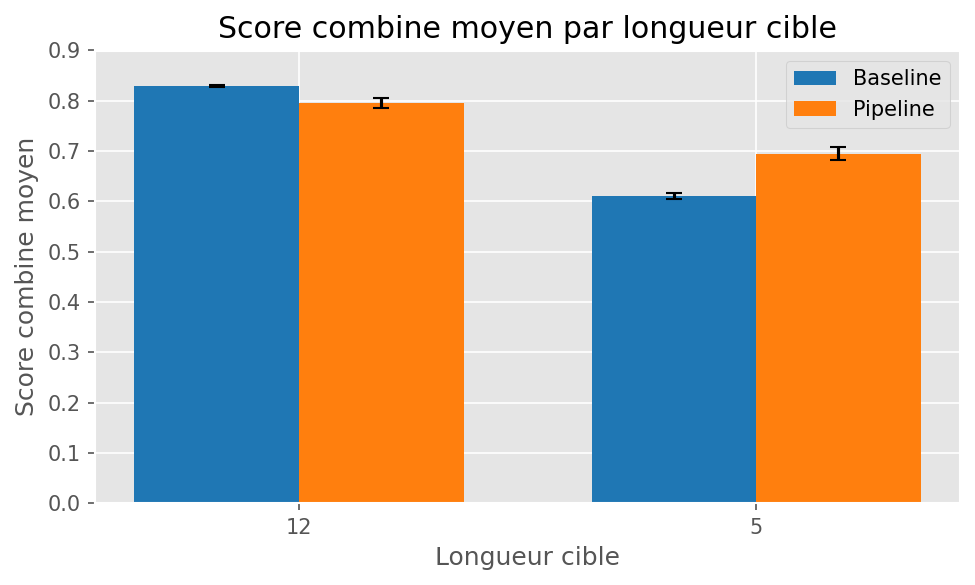
\includegraphics[width=\linewidth]{images/score_per_target_length.png}

        \column{0.5\textwidth}
        \centering
        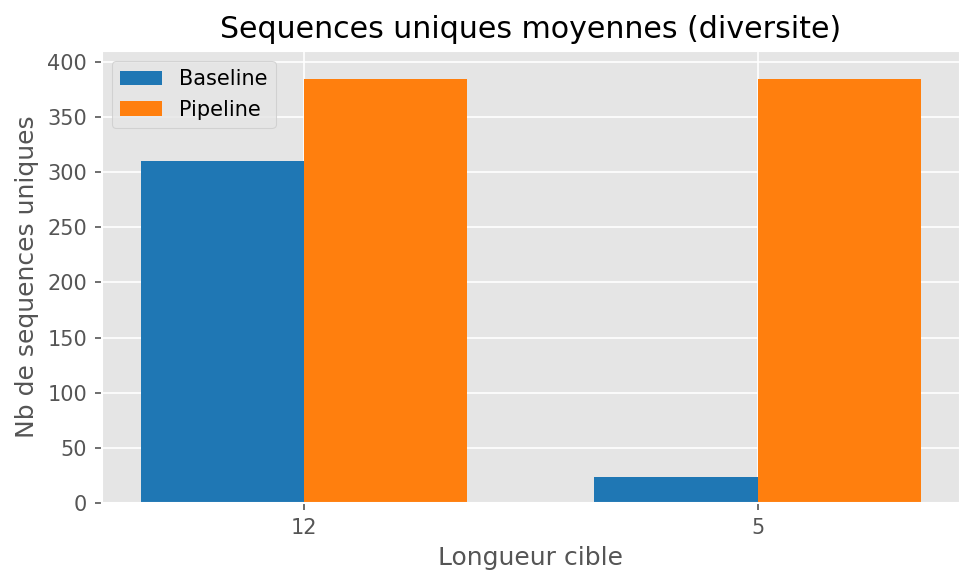
\includegraphics[width=\linewidth]{images/unique_count.png}
    \end{columns}

    \vspace{0.3em}
    \begin{block}{Synthèse}
        \footnotesize
        Le pipeline est \textbf{proche de la baseline} sur cibles longues, mais \textbf{meilleur sur cibles courtes}.
        Côté diversité, le pipeline génère nettement plus de séquences uniques et réduit les duplicats.
    \end{block}
\end{frame}
